%Anexo con imágenes analizadas con algoritmo de procesamiento homomórfico

\begin{figure}[h!]
    \includegraphics[width=0.5\textwidth]{Imagenes/Homomorfico/Paranai1.jpg}
     \hfill
     \caption{Imagen aérea (satelital) de una porción de selva nativa y terrenos cultivados junto al arroyo Paranay }
    %\label{Paranay1}
\end{figure}

\begin{figure}[h!]
    \includegraphics[width=0.5\textwidth]{Imagenes/Homomorfico/Paranai2.jpg}
     \hfill
     \caption{Imagen aérea (satelital) de una porción de selva nativa y terrenos cultivados junto al arroyo Paranay}
    %\label{Paranay2}
\end{figure}

\begin{figure}[h!]
    \includegraphics[width=0.5\textwidth]{Imagenes/Homomorfico/PNI1gris.jpg}
     \hfill
     \caption{Imagen aérea (satelital) Parque Nacional Iguazú, en escala de grises}
    %\label{PNI1}
\end{figure}

\begin{figure}[h!]
    \includegraphics[width=0.5\textwidth]{Imagenes/Homomorfico/PNI2_original.jpg}
     \hfill
     \caption{Imagen aérea (satelital) Parque Nacional Iguazú, en RGB}
    %\label{PNI2}
\end{figure}

\begin{figure}[h!]
    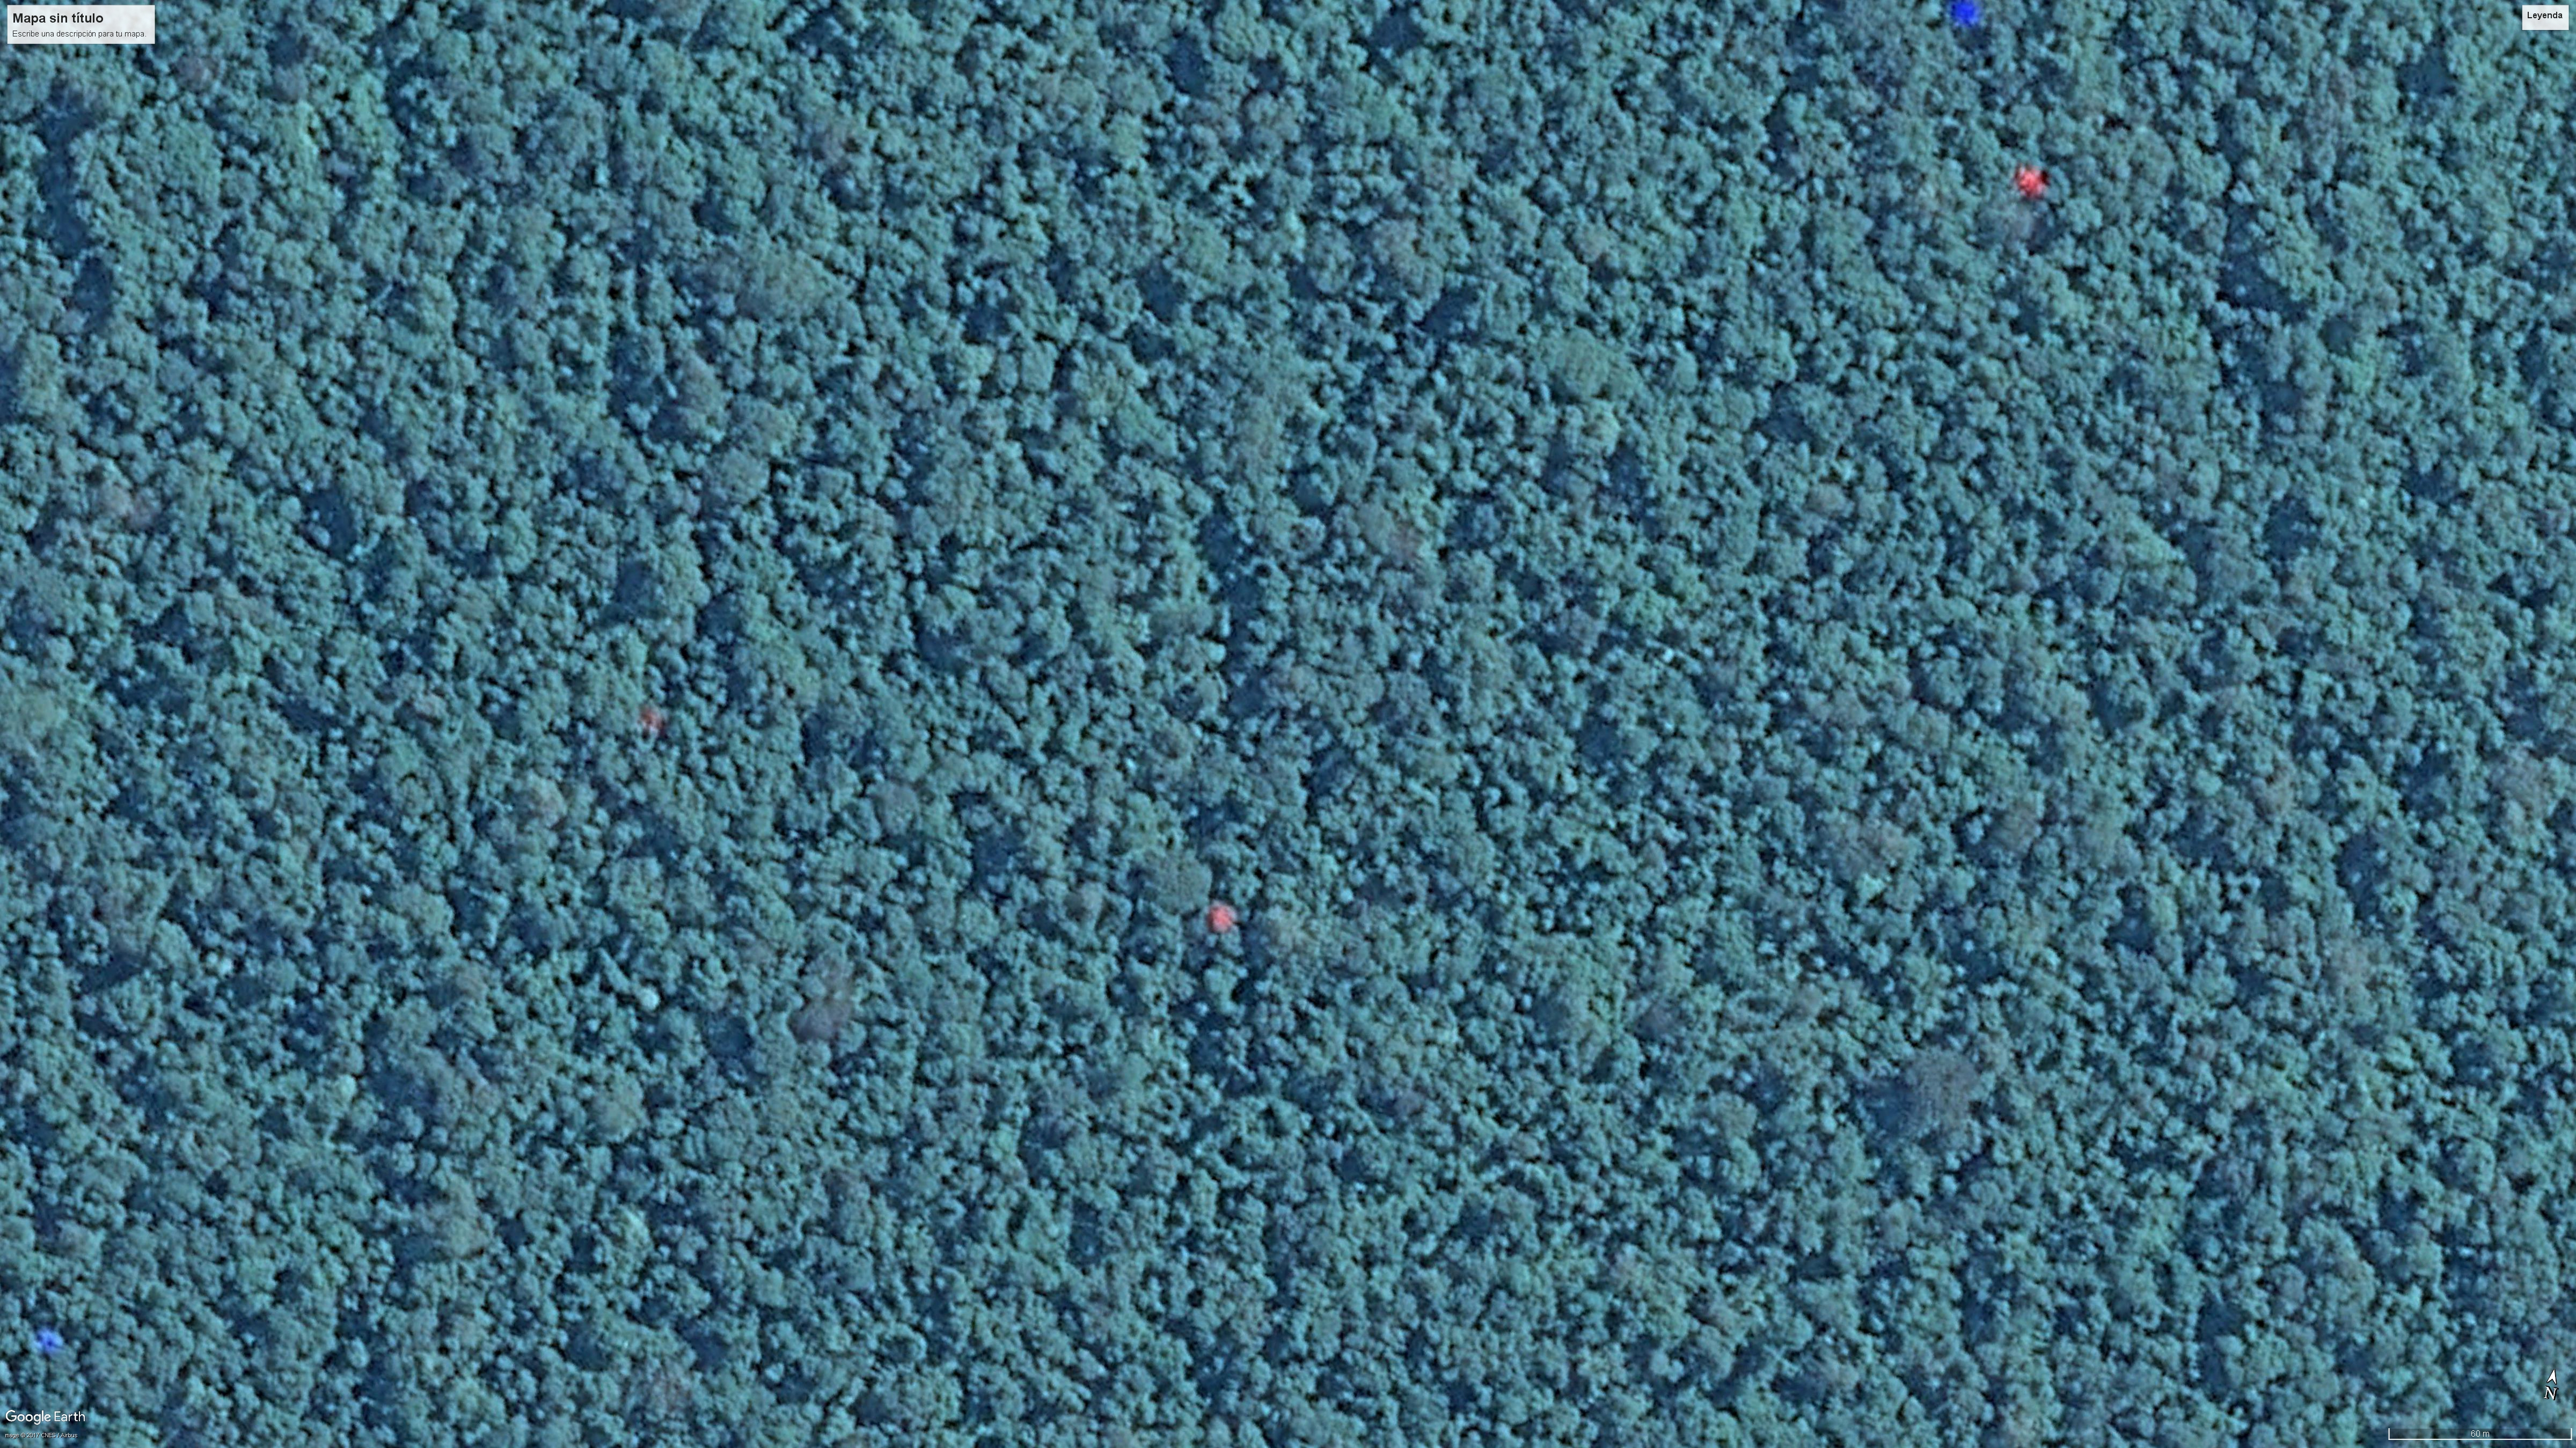
\includegraphics[width=0.5\textwidth]{Imagenes/Homomorfico/PNI_03.jpg}
     \hfill
     \caption{Imagen aérea (satelital) Parque Nacional Iguazú, en RGB}
    %  \label{PNI3}
\end{figure}

\begin{figure}[h!]
    \includegraphics[width=0.5\textwidth]{Imagenes/Homomorfico/PS1_original.jpg}
     \hfill
     \caption{Imagen aérea (satelital) Parque de la Sierra, en RGB}
    %  \label{PS1}
\end{figure}
\begin{figure}[h!]
    \includegraphics[width=0.5\textwidth]{Imagenes/Homomorfico/PS1_bin.png}
     \hfill
     \caption{Imagen binarizada a partir de la imagen \ref{PS1}}
    %  \label{PS1_bin}
\end{figure}
\begin{figure}[h!]
    \includegraphics[width=0.5\textwidth]{Imagenes/Homomorfico/PS1_masked_30.png}
     \hfill
     \caption{Imagen con sombras seleccionadas en forma automática a partir de la imagen \ref{PS1_bin} usando ventana de tamaño 30 x 30 píxeles}
    %  \label{PS1_30}
\end{figure}
\begin{figure}[h!]
    \includegraphics[width=0.5\textwidth]{Imagenes/Homomorfico/YB1.jpg}
     \hfill
     \caption{Imagen aérea (satelital) Biósfera Yaboty, en RGB}
    %  \label{YB1}
\end{figure}
\begin{figure}[h!]
    \includegraphics[width=0.5\textwidth]{Imagenes/Homomorfico/YB2.jpg}
     \hfill
     \caption{Imagen aérea (satelital) Biósfera Yaboty, en RGB}
    %  \label{YB2}
\end{figure}
\begin{figure}[h!]
    \includegraphics[width=0.5\textwidth]{Imagenes/Homomorfico/ST1_gris.png}
     \hfill
     \caption{Imagen aérea (satelital) reserva privada Sombra de Toro, en escala de grises}
    %  \label{ST1}
\end{figure}
\begin{figure}[h!]
    \includegraphics[width=0.5\textwidth]{Imagenes/Homomorfico/ST2.png}
     \hfill
     \caption{Imagen aérea (satelital) reserva privada Sombra de Toro, en RGB}
    %  \label{ST2}
\end{figure}